\documentclass[xcolor=dvipsnames]{beamer}
\usepackage{subfig}
\usetheme{Rochester}  %% Themenwahl
\usecolortheme[named=RoyalBlue]{structure}
\usebackgroundtemplate{
	\centering
	
\includegraphics[width=\paperwidth,height=\paperheight]{images/light-speed}
} 

 \addtobeamertemplate{block begin}{\pgfsetfillopacity{0.5}}{\pgfsetfillopacity{1}}
 \addtobeamertemplate{block alerted begin}{\pgfsetfillopacity{0.5}}{\pgfsetfillopacity{1}}
 \addtobeamertemplate{block example begin}{\pgfsetfillopacity{0.5}}{\pgfsetfillopacity{1}}

\setbeamertemplate{navigation symbols}{}

\title{Solve'n Slide}
\subtitle{Game Prototype}
\author{Hanieh Arjomand-Fard\\Kevin Sawischa\\Markus Ansorge\\Stefan Aicher}
\date{15. May 2017}

\begin{document}
	\maketitle
	\begin{frame}
		\frametitle{Big Idea Bullseye}
		\begin{figure}
			\centering
			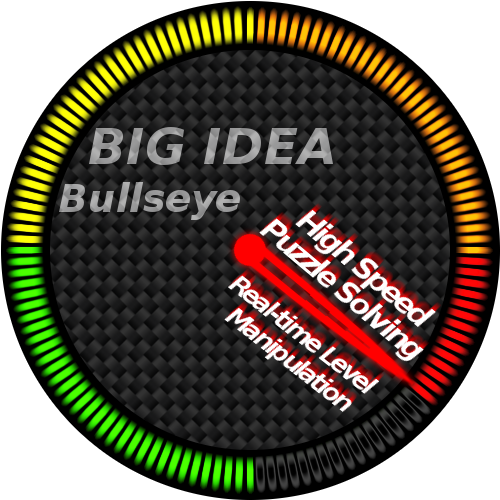
\includegraphics[scale=.4]{images/bigIdeaBullseye}
		\end{figure}
	\end{frame}
	
	\begin{frame}
		\frametitle{Game Idea}
		\begin{itemize}
			%\setlength\itemsep{1.5em}
			\item Two phases
				\begin{itemize}
					\item Manipulation phase
					\item Action phase
				\end{itemize}
			\item Manipulation phase
			\begin{itemize}
				\item Deform terrain to create hills and valleys
				\item Think strategically
				\item Place helpers e.g fuel tanks
				\item consider charges
			\end{itemize}
			\item Action phase
			\begin{itemize}
				\item Slide along self made hills
				\item Take care of obstacles and surfaces of the terrain
			\end{itemize}
		\end{itemize}
	\end{frame}
	
	\begin{frame}
		\frametitle{Prototype - Elements}
		\begin{itemize}
			%\setlength\itemsep{1.5em}
			\item Character represented by a marble
			\item Terrain as a sandbox 75x25x18 cm
			\item Fuel tanks made of paper
			\item Pens marking start and goal point
			\item Using paper as walls
			\item Computer player by one of us
		\end{itemize}
		\begin{figure}[ht]
			\centering
			\begin{tabular}{cc}
				\subfloat{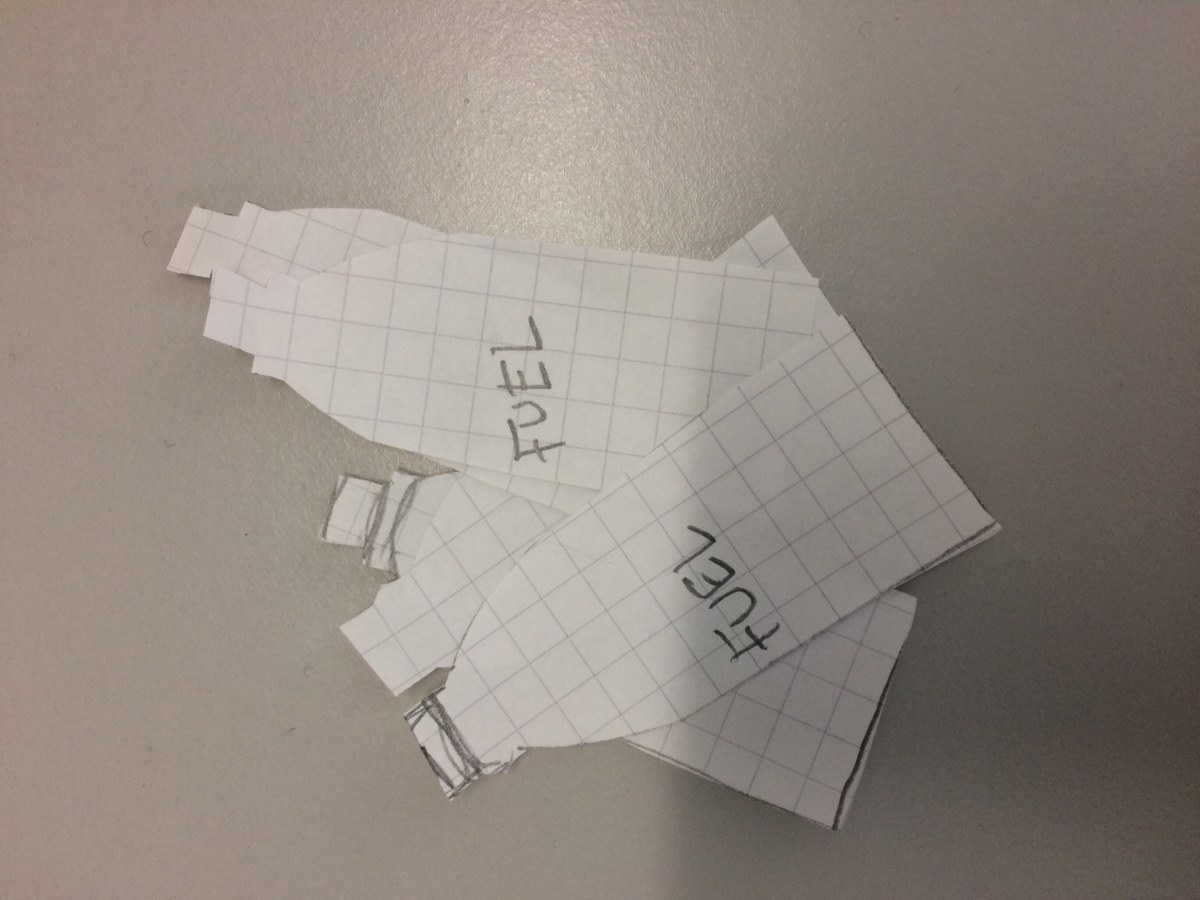
\includegraphics[scale=0.1]{images/prototype/prototypeFuelTanks}}&
				\subfloat{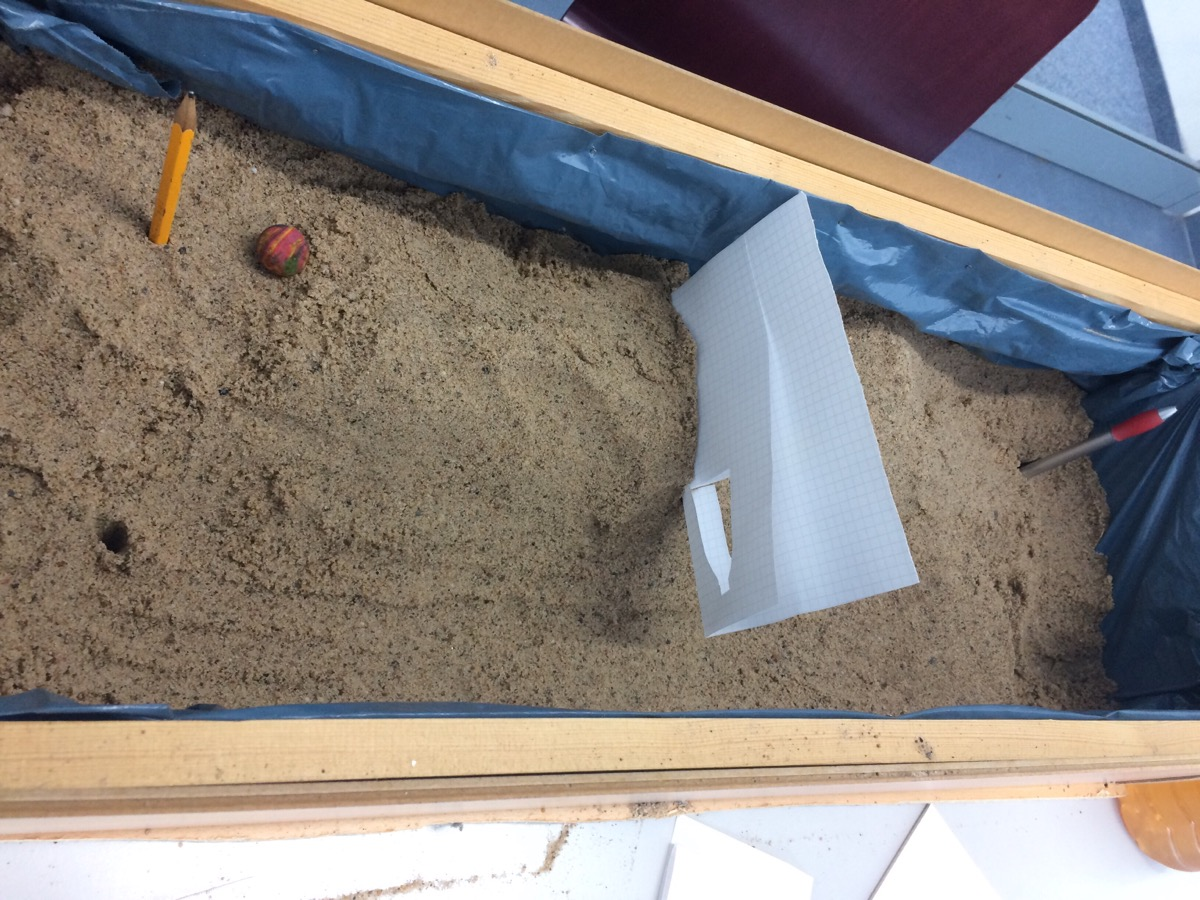
\includegraphics[scale=0.1]{images/prototype/prototypeTerrain2}}
			\end{tabular}
		\end{figure}
	\end{frame}
	
	\begin{frame}
		\frametitle{Prototype - Initialization}
		\begin{itemize}
			\setlength\itemsep{1.5em}
			\item Game is initialized with a default terrain
			\begin{itemize}
				\item Could already have hills, walls and several obstacles
				\item Start and goal point is set
				\item All defined by the whole group except one of us
			\end{itemize}
		\end{itemize}
		\begin{figure}[ht]
			\centering
			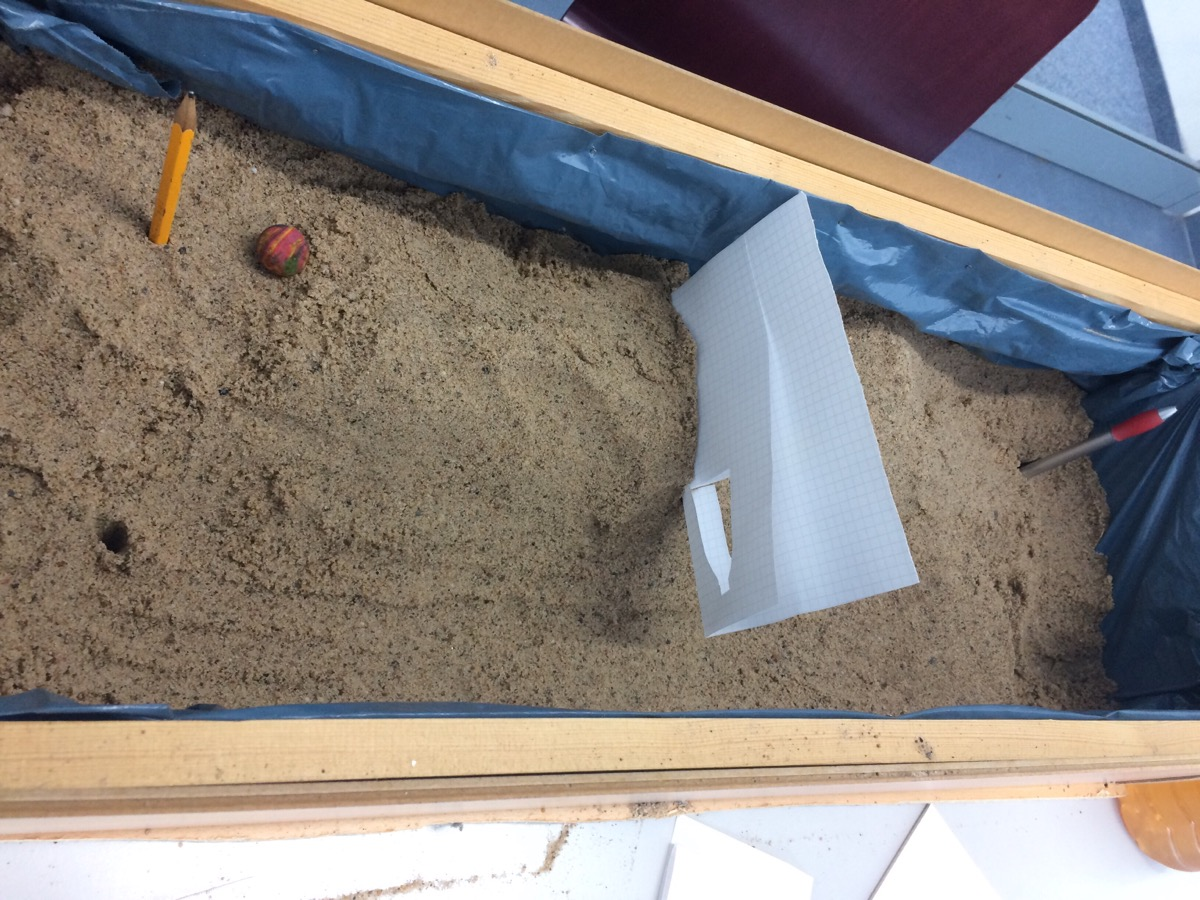
\includegraphics[scale=0.15]{images/prototype/prototypeTerrain2}
		\end{figure}
	\end{frame}
	
	\begin{frame}
		\frametitle{Prototype - Manipulation Phase}
		\begin{itemize}
			\item Player gets the information of how many charges and helpers he gets
			\begin{itemize}
				\item He will get a certain amount of fuel tanks symbolized by paper
			\end{itemize}
			\item Then he starts with the actual game by entering the manipulation phase
			\begin{itemize}
				\item Infinite time to think about how to deform the terrain to his advantage
				\item He picks the place where to raise the terrain and tells it to the computer
				\item Computer executes decisions of the player
				\item On the side player culls spots to player fuel tanks
			\end{itemize}
		\end{itemize}
			\begin{figure}[H]
				\centering
				\begin{tabular}{ccc}
					\subfloat[Step 1]{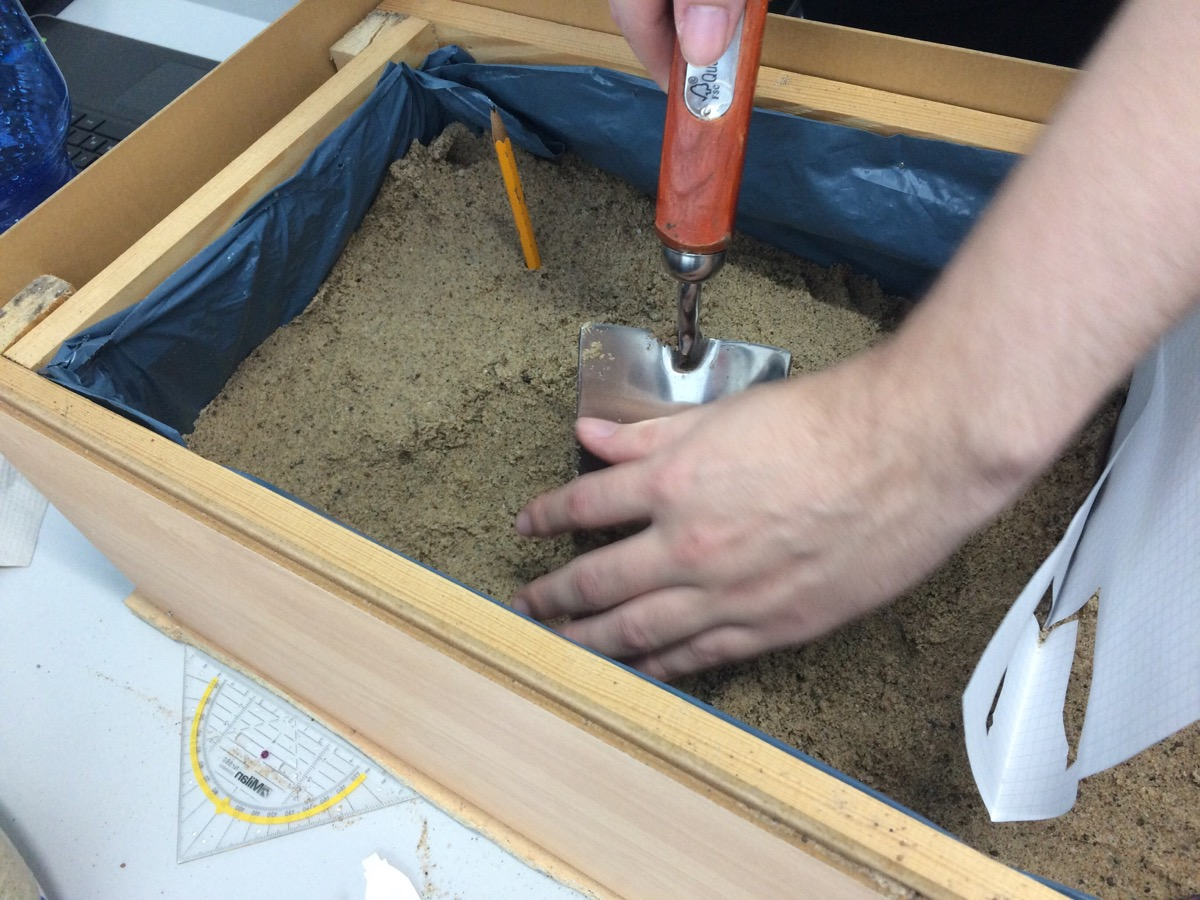
\includegraphics[scale=0.08]{images/prototype/prototypeHill2}}&
					\subfloat[Step 2]{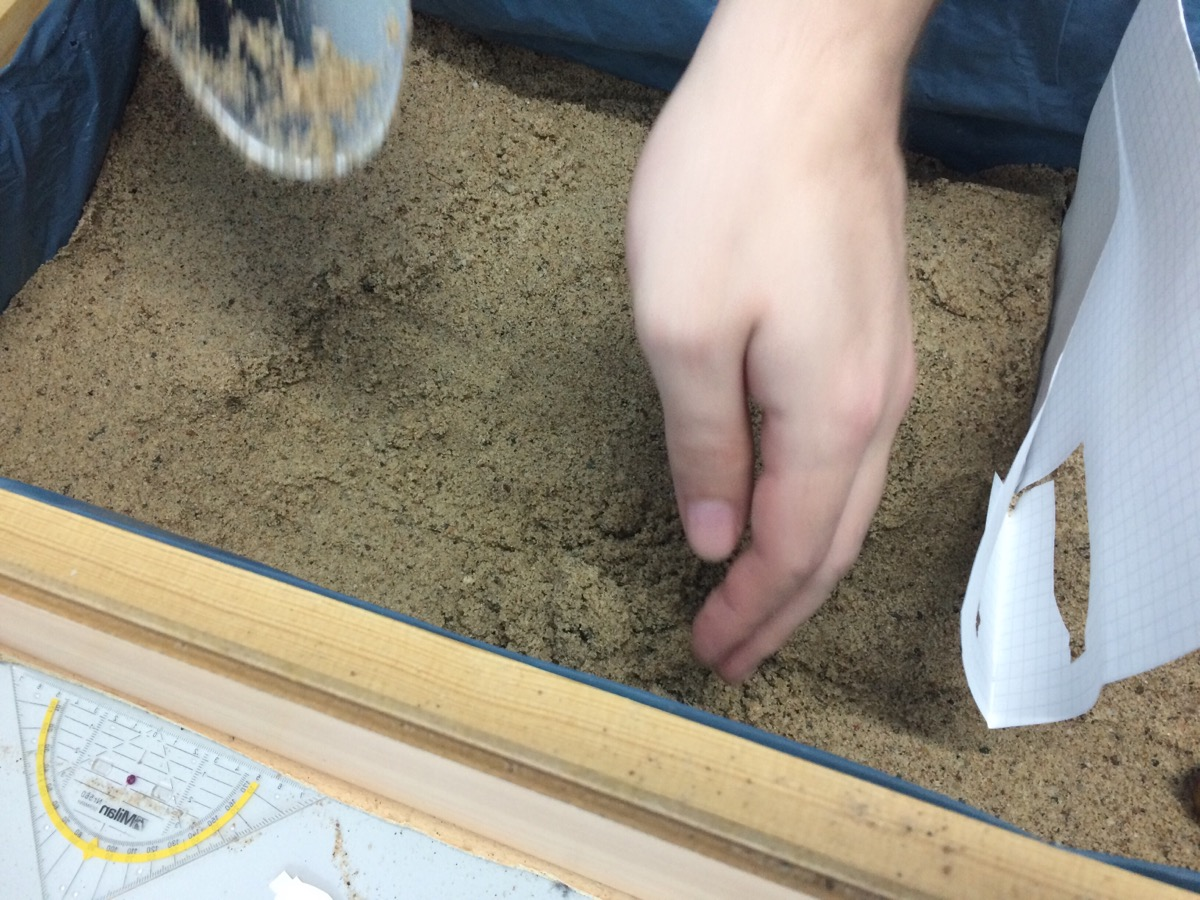
\includegraphics[scale=0.08]{images/prototype/prototypeHill3}}&
					\subfloat[Step 3]{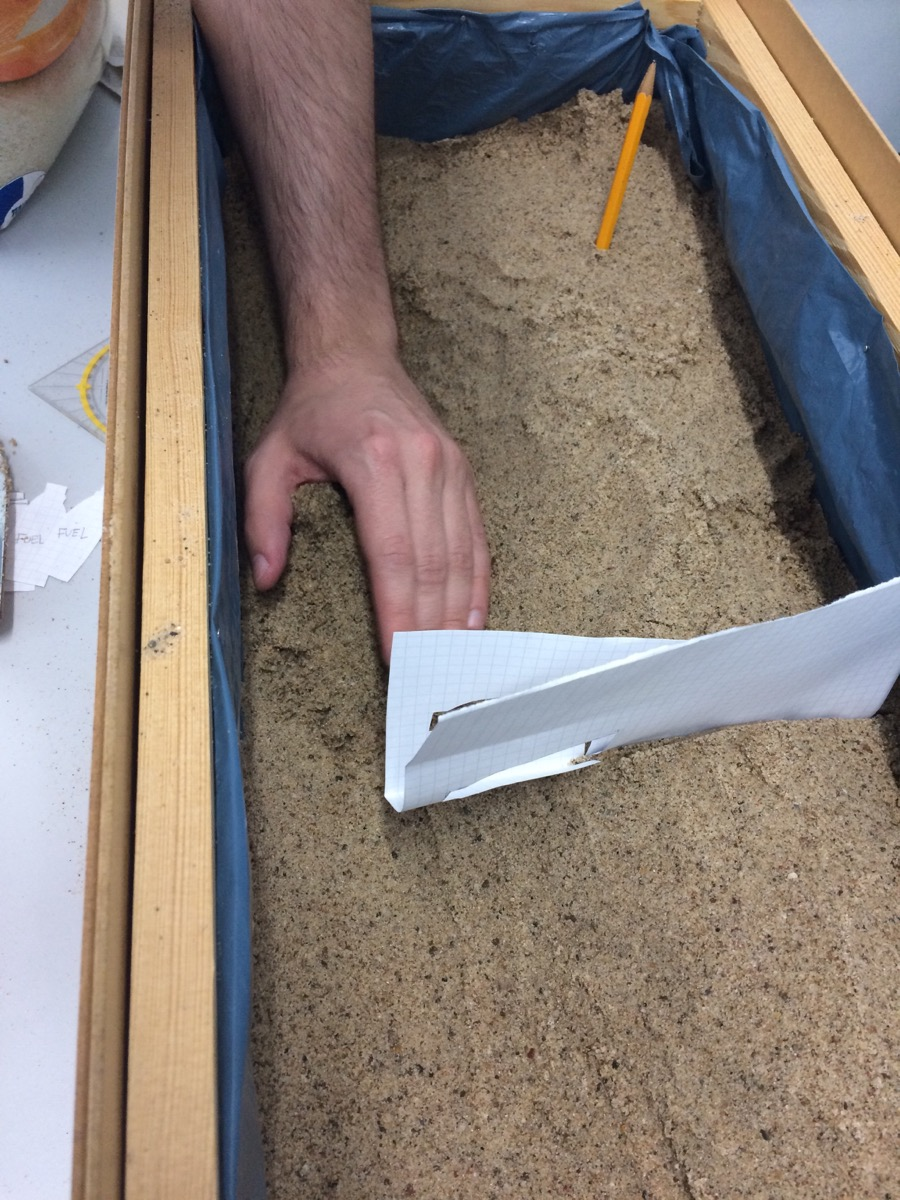
\includegraphics[scale=0.065]{images//prototype/prototypeHill4}}
				\end{tabular}
			\end{figure}
	\end{frame}
	
	\begin{frame}
		\frametitle{Prototype - Action Phase}
		\begin{itemize}
			\item After manipulation, the player enters the action phase
			\item Player/Computer controls the marble
			\item Difficult to simulate momentum and speed
			\item Had to estimate where the marble could land after rolling down a hill
			\item After applying a fuel tank, it was replaced with an empty one
		\end{itemize}
		\begin{figure}[H]
			\centering
			\begin{tabular}{cccc}
				\subfloat[Timestep 1]{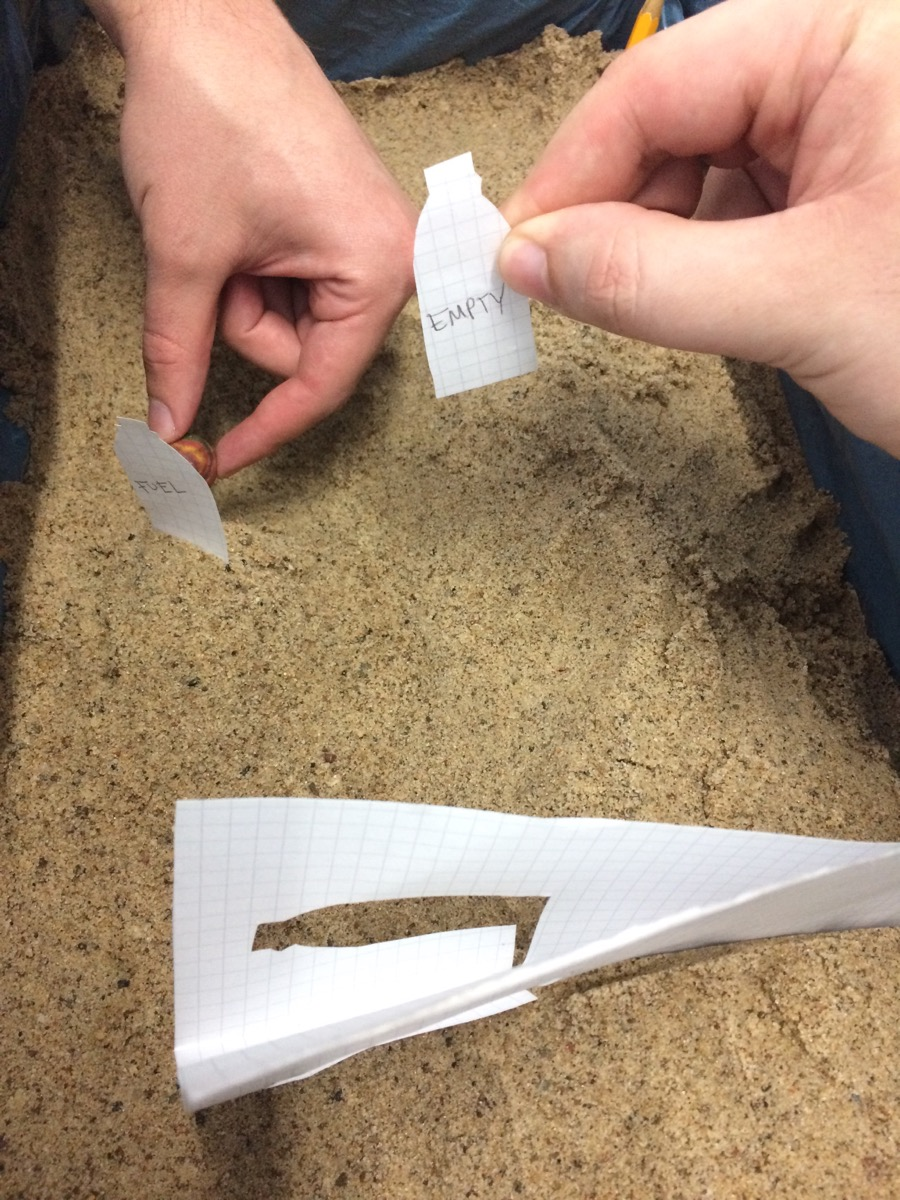
\includegraphics[scale=0.085]{images/prototype/prototypePlaythrough_2_1}}
				\subfloat[Timestep 2]{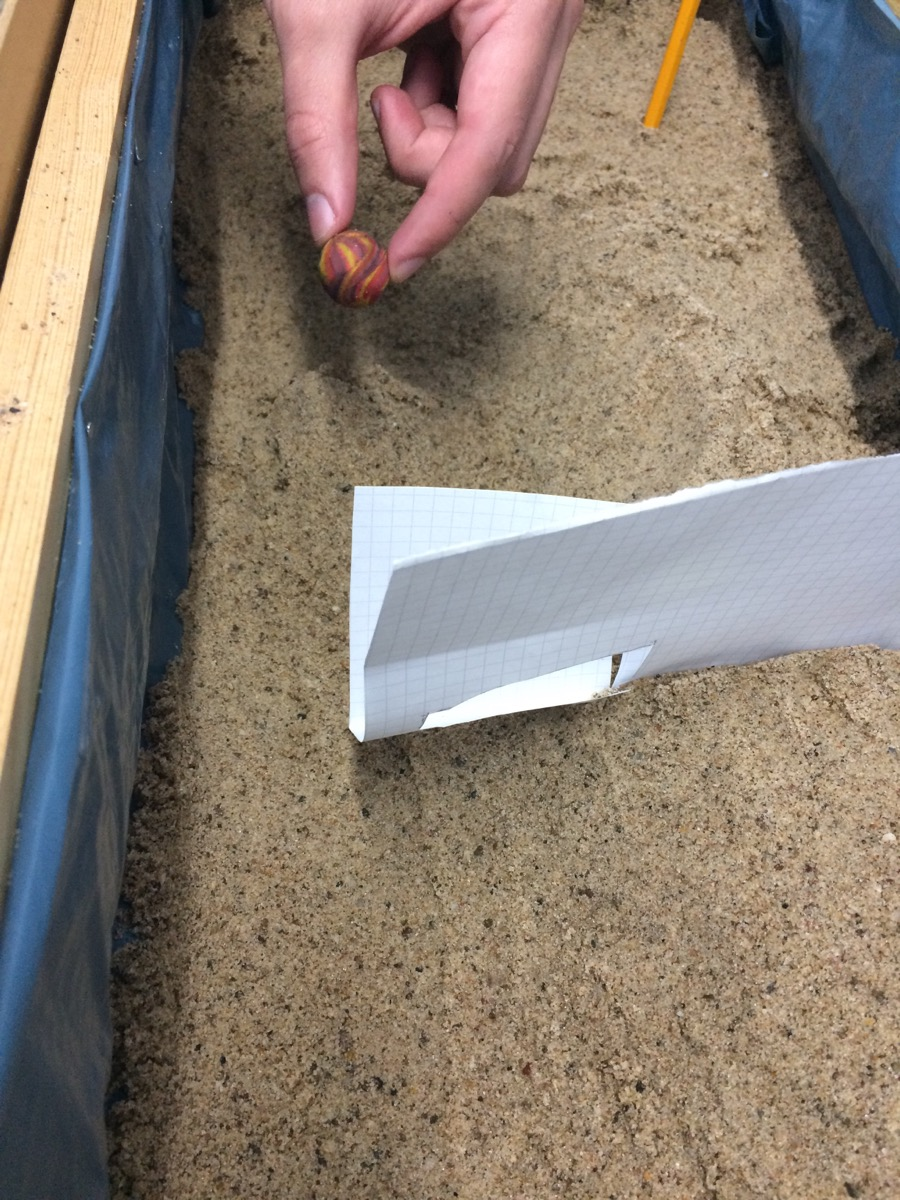
\includegraphics[scale=0.085]{images/prototype/prototypePlaythrough_2_2}}
				\subfloat[Timestep 3]{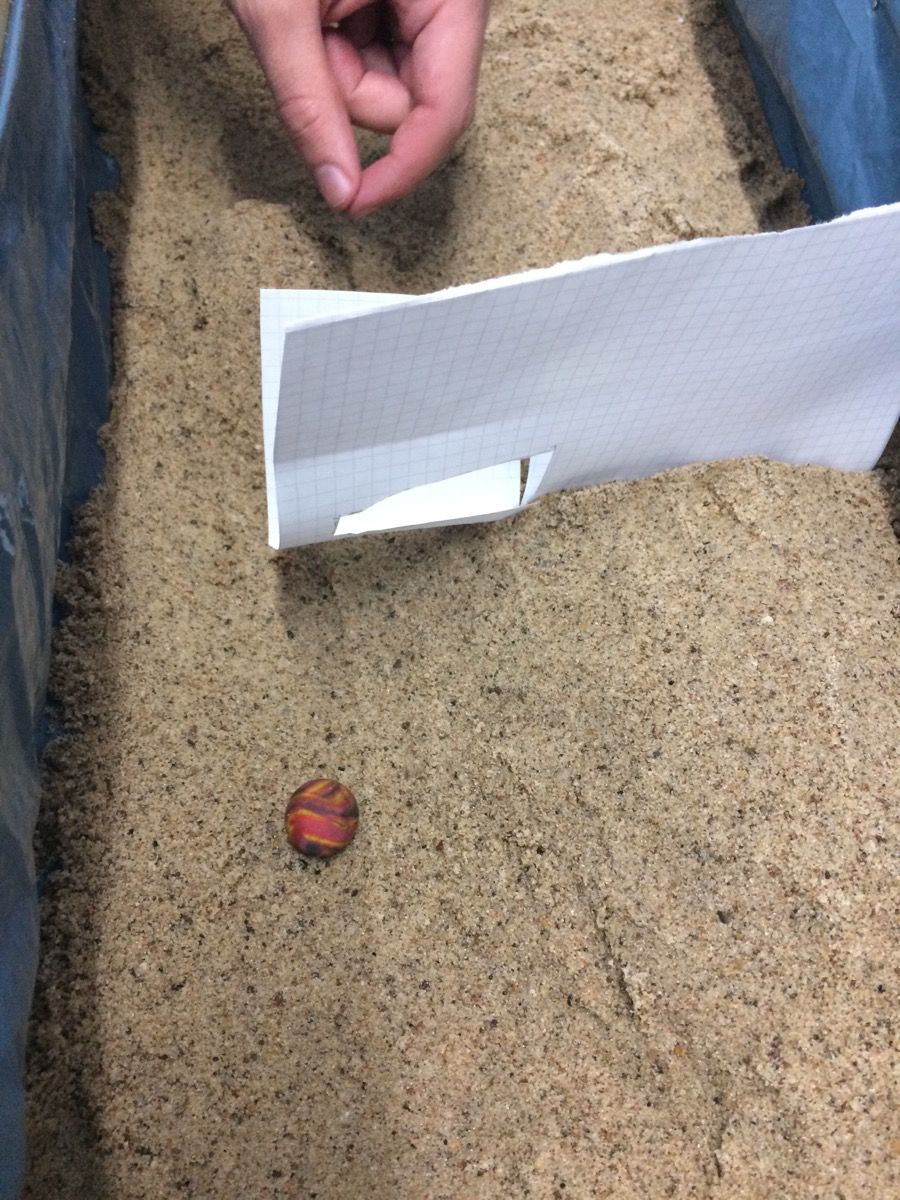
\includegraphics[scale=0.085]{images/prototype/prototypePlaythrough_2_3}}
				\subfloat[Timestep 4]{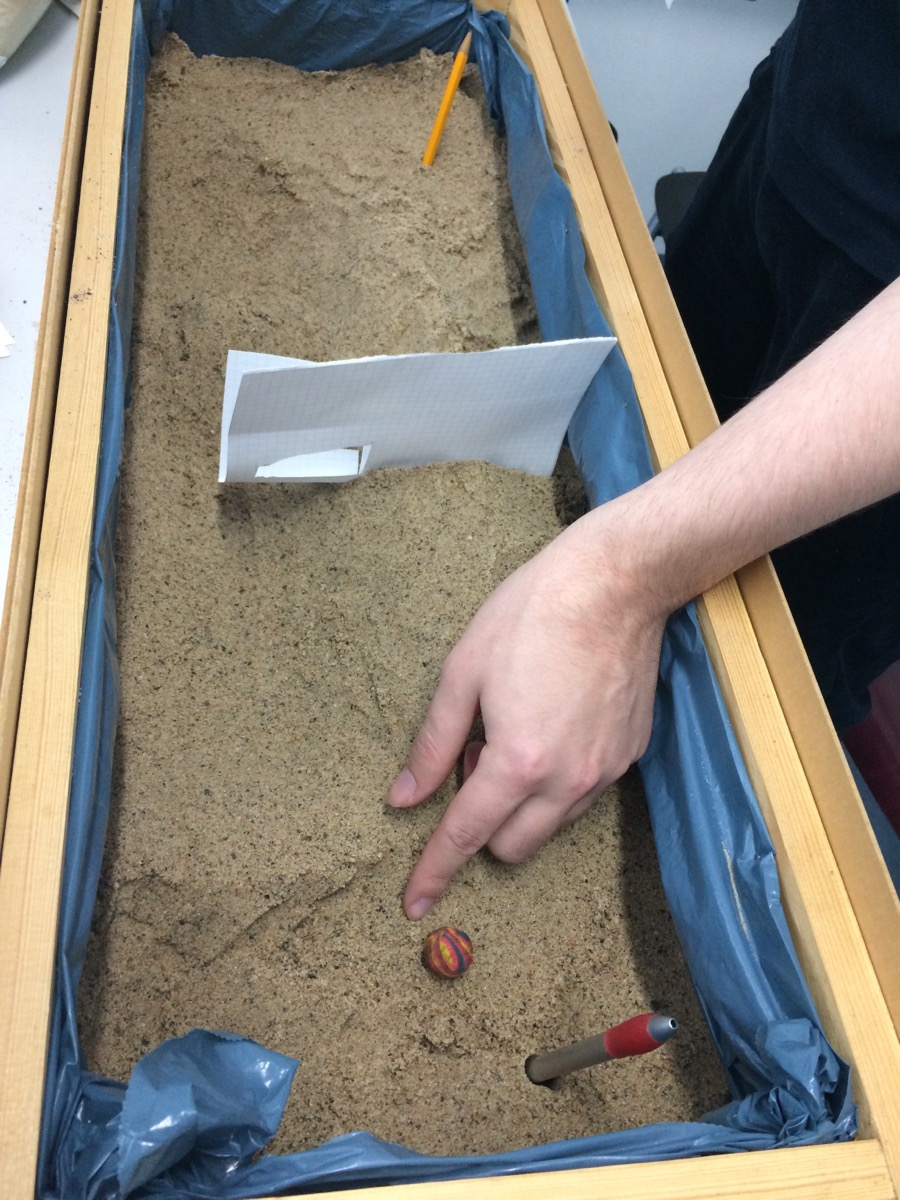
\includegraphics[scale=0.085]{images//prototype/prototypePlaythrough_2_4}}
			\end{tabular}
			\caption{Second Level}
		\end{figure}
	\end{frame}
	
	\begin{frame}
		\frametitle{Why a Sandbox?}
		\begin{itemize}
			\setlength\itemsep{2em}
			\item Manipulation phase almost represented perfectly
			\begin{itemize}
				\item Sand easy to deform
				\item Hills and valleys can be created very flexibly
			\end{itemize}
			\item Action phase was a bit difficult
			\begin{itemize}
				\item High friction decelerated the marble
				\item Only a good estimate when terrain is made of sand in the game as well
			\end{itemize}
			\item But taken as a whole the sandbox was still a good choice since estimating the movements during the action phase would be enough
		\end{itemize}
	\end{frame}
	
	\begin{frame}
		\frametitle{Experience}
		\begin{itemize}
			\setlength\itemsep{5em}
			\item Touching the game idea gives a better feeling of how well our game idea and structure was considered so far
			\item Level design is complexer than we thought
			\begin{itemize}
				\item Design took long
				\item Playing took longer
			\end{itemize}
		\end{itemize}
	\end{frame}
	
	\begin{frame}
		\frametitle{The End}
		\centering
		\Huge
		Thanks for your attention.
	\end{frame}
\end{document}